\chapter{Iteración I: “Despliegue e instalación de Security Onion en un ambiente de prueba”}
    En este capítulo describiremos la instalación de Security Onion en la topología de la red de prueba seleccionada. Se instalará un nodo Master, dos nodos Forward y un nodo de TheHive. \par
    En este proyecto se desarrolló sobre un ambiente de prueba primero y de producción después. Se utilizo un servidor central y un sistema operativo de virtualización sobre el que se crearon un conjunto de máquinas virtuales, cada una alojando un servidor con nodos Forward, Master y el correspondiente a TheHive - Cortex. Se utilizó de guía los componentes, el software y la arquitectura de conexión entre ellos, mencionados en la Descripción de Security Onion.

    
    \begin{section}{Selección de hardware} 
        El primer paso consistió en examinar los requisitos de hardware mínimos y recomendados por cada uno de los fabricantes de los sistemas y subsistemas elegidos. Se analizaron, por un lado, las demandas de tráfico de red en el ambiente de prueba y por el otro los requerimientos sobre los datos y capacidades que se esperan obtener del proyecto. Se realizó un diagrama topológico en la infraestructura objetivo, con esta información y los datos anteriormente mencionados, se dimensiono el hardware necesario para el servidor central, que albergó las correspondientes máquinas virtuales de este proyecto.\par
        Según el fabricante, los requerimientos de hardware para un entorno de producción con enlaces de 1 Gbps son son los que figuran en el Cuadro \ref{table:5}.
        
        \begin{table}[H]
        \centering
        \begin{tabular}{|m{9em}|m{9em}|m{9em}|m{9em}|}
        
            \hline 
                Requerimiento  & Nodo Master &  Nodo Forward & TheHive y Cortex \\ 
            \hline
                Cantidad de CPU - Arquitectura & Mínimo de 8 núcleos vCPU - x86-64 & Mínimo de 12 núcleos vCPU - x86-64 & Mínimo de 8 núcleos vCPU - x86-64 \\ 
            \hline
                Memoria RAM  & 12 a 128 GB & 128 a 256 GB & A partir de 8 GB \\ 
            \hline
                Almacenamiento necesario & Mínimo de 1 TB  & Mínimo de 540 GB & A partir de 60 GB \\
            \hline %linea final de tabla
        \end{tabular}
        \caption{Requerimientos de hardware recomendados por el fabricante para el monitoreo de un enlace de 1 Gbps}
        \label{table:5}
        \end{table}
        
        Debido a las restricciones en la disponibilidad del hardware, se realizó una implementación aproximada, teniendo en cuenta la optimización al máximo de los recursos disponibles. \par
	    Los nuevos requerimientos de hardware que se utilizaron se incluyen en el Cuadro \ref{table:12}.

        \begin{table}[H]
        \centering
        \begin{tabular}{|m{9em}|m{9em}|m{9em}|m{9em}|}
        
            \hline 
                Requerimiento  & Nodo Master &  Nodo Forward & TheHive y Cortex \\ 
            \hline
                Cantidad de CPU - Arquitectura & 8 nucleos vCPU - x86-64 & 10 nucleos vCPU - x86-64 & 8 nucleos vCPU - x86-64 \\ 
            \hline
                Memoria RAM  & 16 GB & 32 GB & 8 GB \\ 
            \hline
                Almacenamiento necesario & 500 GB  & 200 GB & 60 GB \\
            \hline %linea final de tabla
        \end{tabular}
        \caption{Requerimientos de hardware según el tipo de nodo desplegado. Los requerimientos varían según el tipo de enlace a monitorear.}
        \label{table:12}
        \end{table}
        \FloatBarrier
        %En este proyecto se monitorearon enlaces de 1 Gbps de ancho de banda, por lo tanto los requerimientos para el nodo forward se incrementaron a 10 núcleos vCPU y 32 GB de memoria RAM. \par
        En cuanto a los núcleos de CPU virtuales, su frecuencia era de 2.4 Ghz, basados en procesadores físicos Intel Xeon E5620. Las memorias RAM pertenecían a la tecnología DDR3 y su frecuencia de refresco de 2400 MHz.
        Los discos eran del tipo mecánico con una velocidad de transferencia para lectura de 196 MB/s y para escritura de 154 MB/s, con interfaz SATA III y 7200 rpm de velocidad de rotación. \par
    	Se optimizó al máximo el uso de los recursos del servidor disponible para permitir el despliegue de cuatro nodos: dos Forward y un Master de Security Onion, así como un cuarto conteniendo a TheHive y Cortex. \par

        \begin{subsection}{Configuración del entorno de virtualización}
        Para el entorno de virtualización se utilizó VMWare \cite{vmware}, concretamente la suite vSphere HyperVisor v6.7.0 u3. Este sistema operativo basado en Unix permite gestionar los recursos de hardware disponibles, almacenar imágenes de distintos sistemas operativos y crear máquinas virtuales con estos últimos. Durante el proceso de creación de una máquina virtual, se selecciona el sistema operativo deseado y es posible asignar distintas cantidades de memoria principal, secundaria, cantidad de vCPU, número y tipo de enlaces de red, entre otros parámetros. \par
         \begin{figure}[H]
          \centering
           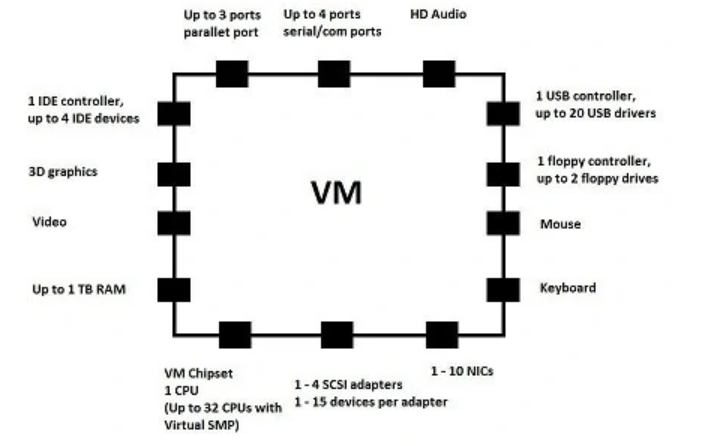
\includegraphics[width=0.7\textwidth]{./iteracion_1_imagenes/figura_34_diagrama_VM.png}
            \caption{ Diagrama de una máquina virtual desde el punto de vista de un HyperVisor\cite{vmware}}
            \label{fig:maquina_virtual}
        \end{figure}
        \end{subsection}
        
        \begin{subsection}{Definición y configuración de las redes a observar}
            Se decidió monitorear dos dependencias en base a un análisis del ancho de banda de las dependencias existentes. Se seleccionaron las que mayor volumen de tráfico registraban en función de un registro histórico y mediciones propias realizadas a lo largo de una semana. Las dependencias seleccionadas tenían un enlace con ancho de banda de 1 Gbps cada una, con  velocidades promedio consideradas como la suma entre entrada y salida, entre 11,95 y 47,24 Mbps respectivamente; con picos poco frecuentes de 300 Mbps de tráfico, que no se contemplaron en los requisitos de hardware, por lo tanto habrá una posible pérdida de paquetes en estos casos. Se realizó un “port mirroring” de los puertos del switch capa 3 a los que están conectados estas dependencias y se los conecto con los respectivos enlaces de monitoreo de sendos nodos Forward de Security Onion. \par
            Las Figuras \ref{fig:figura_35_trafico_dia} y \ref{fig:figura_36_trafico_semana} fueron tomadas usando LibreNMS\cite{librenms} (versión 1.48)  muestran el volumen del tráfico medido en dos periodos de tiempo distintos: Durante un día (exceptuando las horas en las que la actividad era mínima) y a lo largo de una semana. Si bien estos registros que se presentan a continuación corresponden a una sola de las dependencias, la restante tenía un comportamiento análogo. \par
            
            \begin{figure}[H]
                \centering
                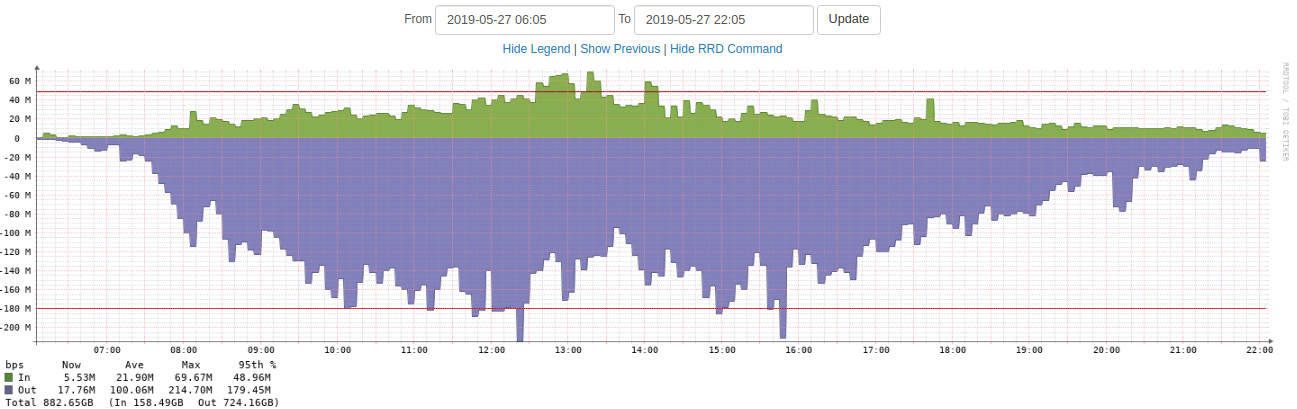
\includegraphics[width=1\textwidth]{./iteracion_1_imagenes/figura_35_trafico_dia.png}
                \caption{Tráfico correspondiente a una dependencia, medido durante un día, obviando las horas donde este es casi nulo}
                \label{fig:figura_35_trafico_dia}
            \end{figure}
            \begin{figure}[H]
            \centering
            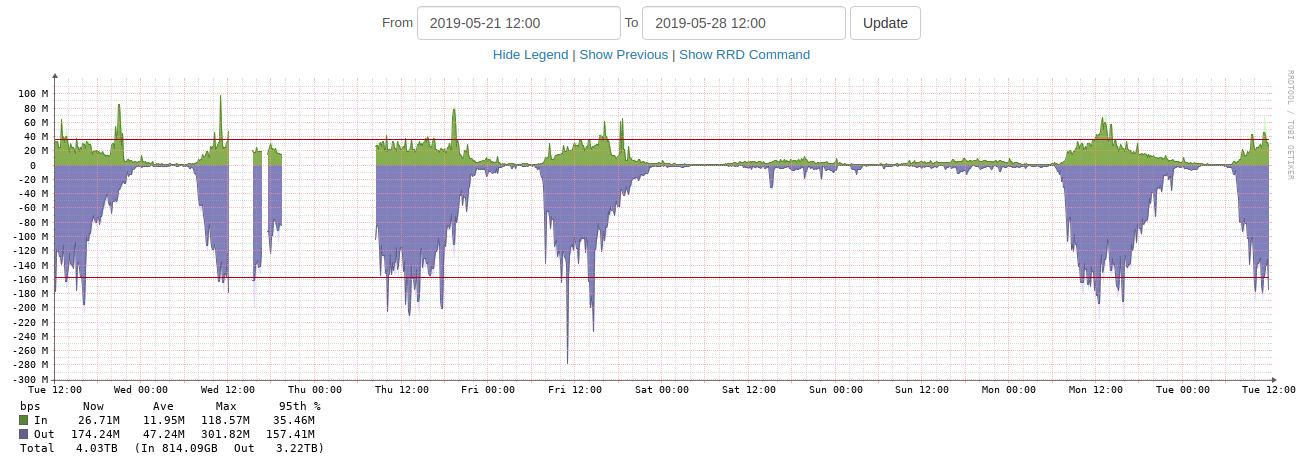
\includegraphics[width=1\textwidth]{./iteracion_1_imagenes/figura_36_trafico_semana.png}
            \caption{Tráfico medido durante el periodo correspondiente a una semana}
            \label{fig:figura_36_trafico_semana}
            \end{figure}
        \end{subsection}
    \end{section}
    
    \begin{section}{Configuración inicial del sistema base}
        Es posible instalar Security Onion en su versión 16.04 de dos maneras: mediante una ISO provista por los desarrolladores o bien mediante una serie de paquetes en una distribución Ubuntu \cite{ubuntu}. En este último caso será necesario contar con la distribución Ubuntu en su versión 16.04, ya que las distribuciones de Security Onion siguen a las distribuciones respectivas de Ubuntu. A partir del año 2020 se lanzaron nuevas versiones de Security Onion con soporte a otras distribuciones Linux: CentOS 7 y Ubuntu 18.04 y 20.04, aunque en el futuro se podrá desplegar en otros tipos de sistema Linux. Desde la versión 2.x de Security Onion en adelante, el sistema se despliega en contenedores.

        \begin{subsection}{Instalación y configuración de Security Onion}
        Como se mencionó en la sección anterior, existen dos maneras de instalar esta versión de Security Onion: a partir de una imagen ISO o mediante paquetes. \par 
        Si la instalación de Security Onion fue realizada mediante una ISO, luego de finalizada es necesario elegir el rol (Master o Forward) del nodo mediante el asistente y a continuación realizar la configuración del mismo. Para esto último, se cuenta con la guía del asistente integrado que permite elegir y configurar las interfaces disponibles (observación o administración). \par
        Al finalizar el proceso y si se trata de un nodo Forward, el asistente pedirá elegir el motor IDS (Snort o Suricata). El último paso consiste en elegir entre dos tipos de modo de funcionamiento: Producción o Evaluación.\par
       
        A fin de realizar pruebas iniciales del sistema, se eligió la primer opción. Posteriormente, cuando se comprobó el funcionamiento de la mayoría de sus componentes, se desplegó el sistema mediante paquetes de la distribución 16.04 de Security Onion. Esta decisión se tomo debido a una solicitud de la organización, ya que esta contaba con maquinas virtuales configuradas con Ubuntu 16.04. \par
        
        Se dispuso de un sistema operativo Ubuntu Server 16.04 con la particularidad de tener dos discos montados: el principal para el sistema operativo y el secundario para los datos recolectados en un directorio \textbf{/nsm}. En el caso de un servidor Master se almacenan índices en este directorio. En el caso de un nodo Forward, en el directorio \textbf{/nsm} se almacenan capturas de paquetes o logs. \par 
        
        
        Sin importar el método de instalación, al finalizar el proceso, las configuraciones se pueden llevar a cabo mediante el comando \textit{sosetup -f $\sim$/sosetup.conf}. Esta instrucción ejecuta un programa que lee las configuraciones previamente guardadas en un archivo.
         \begin{figure}[H]
            \centering
            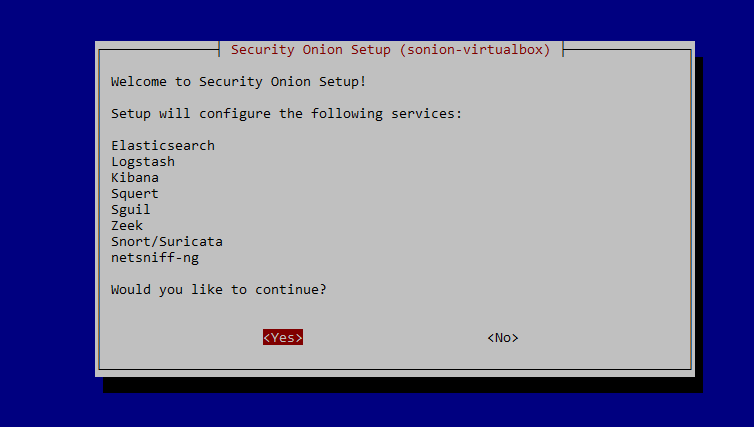
\includegraphics[width=0.7\textwidth]{./iteracion_1_imagenes/figura_37_sonion_conf.png}
            \caption{Asistente de instalación de Security Onion 16.04}
            \label{fig:figura_37_sonion_conf}
        \end{figure}
        \begin{figure}[H]
            \centering
            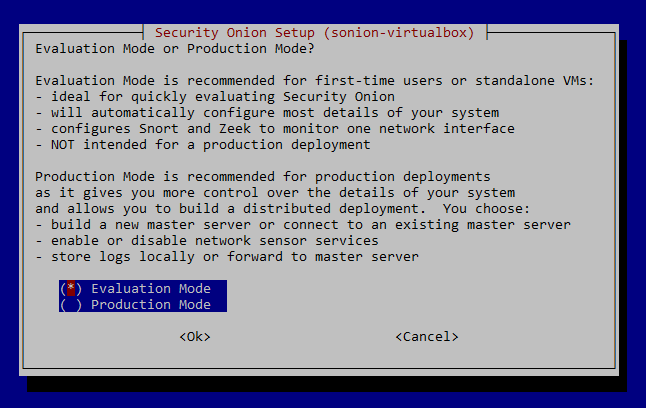
\includegraphics[width=0.7\textwidth]{./iteracion_1_imagenes/figura_38_sonion_modo.png}
            \caption{El asistente de instalación permite elegir el modo de despliegue}
            \label{fig:figura_38_sonion_modo}
        \end{figure}
        Con el objetivo de cumplir uno de los requerimientos no funcionales del proyecto, que implica la automatización del despliegue (instalación y configuración) del sistema, se utilizó una herramienta de administración automatizada de servidores llamada Ansible en su versión 2.8.4 para la cual se desarrollaron scripts YAML conteniendo la secuencia de instalación de los paquetes, configuraciones, rol del nodo (Forward o Master) y librerías requeridas para el apropiado funcionamiento del sistema.
        \end{subsection}
        
      
   
   
   
   
        \begin{subsection}{Instalación y configuración de TheHive - Cortex}
        Para la instalación del gestor de incidentes, que tiene como componentes a  TheHive y Cortex, se utilizó  el sistema operativo Debian 10. En primer lugar se instaló TheHive, para ello fue necesario realizar la instalación previa de los componentes necesarios como las librerías de Java, Python y Elasticsearch; este último requirió una configuración en su archivo elasticsearch.yaml:
        
        \begin{figure}[H]
            \centering
            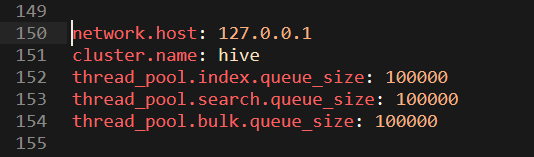
\includegraphics[width=0.7\textwidth]{./iteracion_1_imagenes/figura_39_thehive_conf_elastic.png}
            \caption{Configuración añadida a elasticsearch.yaml para la instalación de TheHive}
            \label{fig:figura_39_thehive_conf}
        \end{figure}
        Finalmente, los últimos pasos para la instalación de TheHive consisten en habilitar e iniciar el servicio de elasticsearch, agregar el repositorio que contiene los paquetes de TheHive, instalarlo y luego habilitar el servicio para poder iniciarlo. \par
        En cuanto a Cortex, el proceso es similar al anteriormente descrito para TheHive, donde una vez descargados e instalados los paquetes de Cortex con su correspondiente secuencia de habilitación e inicio; se procedió a descargar del repositorio los responders y analyzers respectivos. Por último, se modifica el archivo de configuración de Cortex para indicar la ubicación del directorio que contiene los responders y analyzers mencionados anteriormente. \par
        Posteriormente se actualizó la base de datos elasticsearch mediante la GUI web de Cortex, se creó un superusuario y luego las organizaciones donde se administrarán usuarios comunes y analyzers; es necesario crear un usuario con el rol de administrador de organizaciones. Las organizaciones tendrán habilitados y configurados determinados responders y analyzers según sea necesario. \par
        El último paso del proceso consiste en comunicar TheHive y Cortex entre sí. Para ello se genera una API key en Cortex que será usada como parte de las modificaciones necesarias al archivo application.conf de TheHive. Las modificaciones completas que se realizaron al mencionado archivo se pueden apreciar en la Figura \ref{fig:figura_40_thehive_cortex_conf}:\par
        
        \begin{figure}[H]
            \centering
            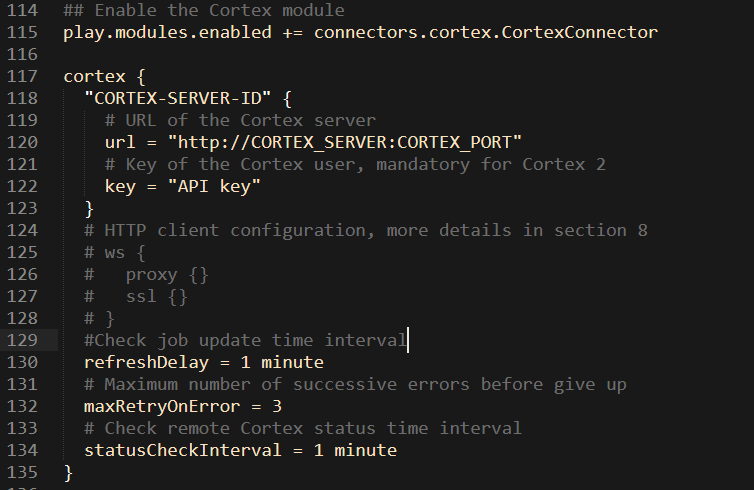
\includegraphics[width=0.7\textwidth]{./iteracion_1_imagenes/figura_40_thehive_cortex_conf.png}
            \caption{Modificación al archivo application.conf de TheHive para la comunicación con Cortex}
            \label{fig:figura_40_thehive_cortex_conf}
        \end{figure}
        \end{subsection}
    \end{section}
    
    
    \begin{section}{Topologías de red }
        Durante el desarrollo de este proyecto, se evaluaron dos tipos de topologías de red. En primer lugar se ensayo con un tipo de topología monolítica que concentraba todos los componentes esenciales de Security Onion. Si bien se conocía que el rendimiento no era óptimo, se decidió comenzar por este punto para evaluar inicialmente al sistema. \par
        Con el conocimiento adquirido sobre la naturaleza de Security Onion, se procedió a experimentar y finalmente desplegar en producción, versiones correspondientes a topologías distribuidas de la solución. \par

        \begin{subsection} {Topología Monolítica}
            Con motivo de familiarizarnos con Security Onion, se decidió desplegar este tipo de topología para facilitar la comprensión del funcionamiento de sus componentes. Se realizaron pruebas de los requerimientos funcionales 1 y 3: se comprobó la capacidad de recolectar y almacenar datos de incidentes de seguridad en la infraestructura de red de la organización, al enviar PCAPS e información previamente generadas de ataques que había sufrido la organización en el pasado. Se pudo observar estos eventos en un panel de mando, con lo que se verificó el cumplimiento del requisito funcional 3.\par 
            En la Figura \ref{fig:figura_33_a}, se observa una típica topología de red en el cual se despliega la solución con una arquitectura monolítica. En el switch se encuentran conectadas dos terminales y el nodo monolítico de Security Onion. Una terminal simula ser la de un analista consultando y visualizando datos en Security Onion, mientras que la terminal restante envía logs mediante Filebeat \cite{filebeat}, conteniendo información contextual de los activos de la red. Esto permite cumplir el requerimiento funcional 2, que sera tratado y demostrado en la Iteración II (Capitulo \ref{iteracion2}). 
            \begin{figure}[H]
            \centering
            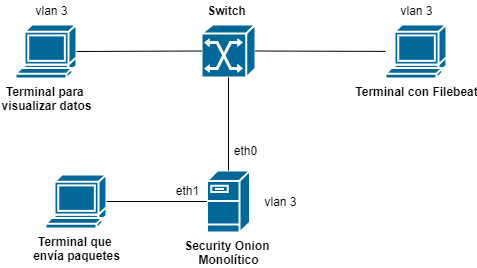
\includegraphics[width=0.7\textwidth]{./iteracion_1_imagenes/figura_33_a_topologia_de_prueba_1.png}
            \caption{Topología monolítica}
            \label{fig:figura_33_a}
            \end{figure}
            El nodo monolítico de Security Onion dispone de dos conexiones. La correspondiente al puerto eth0 es la que permite la administración del sistema y la consulta de sus datos, mientras que la interfaz eth1 es la destina a monitorear el tráfico de una red. En nuestro experimento con esta arquitectura, todo el tráfico fue simulado usando los PCAPS mencionados anteriormente. \par
            Este tipo de topología es ineficiente para el uso en entornos de producción, dado que la pila Elastic y los componentes de los sensores IDS demandan un uso intensivo de hardware. Por esta razón se procedió a analizar el despliegue de una topología distribuida.
            \par
            En la siguiente sección (\ref{subsection:topo_dist}) se demuestra el cumplimiento de los requerimientos funcionales 1 y 3.
        \end{subsection}
        \begin{subsection} {Topología Distribuida}
        \label{subsection:topo_dist}
            Después de comprobar el funcionamiento de los principales componentes de Security Onion y obtener la experiencia descrita en la sección anterior, se procedió a considerar el despliegue de una topología distribuida. Este tipo de topología presenta considerables ventajas respecto de su alternativa monolítica, fundamentalmente en términos de rendimiento del hardware y flexibilidad de adaptación, tal como se mencionó en el Capítulo  \ref{tipos_de_arquitectura}. \par
            En primer lugar, se desplegó una versión simplificada para verificar el funcionamiento de los componentes de los dos nodos que la componen (nodos Forward y Master) y la comunicación entre ellos.\par
            \begin{figure}[h]
                \centering
                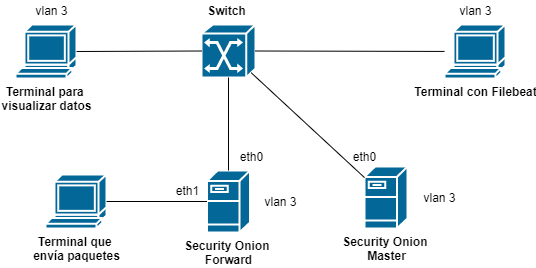
\includegraphics[width=1\textwidth]{./iteracion_1_imagenes/figura_33_b_topologia_de_prueba_2.png}
                \caption{Versión elemental de una topología distribuida}
                \label{fig:topologia_distribuida_1}
            \end{figure}
            \FloatBarrier
            Se observa en la Figura \ref{fig:topologia_distribuida_1} los componentes fundamentales de Security Onion para poder llevar a cabo esta topología: un nodo Forward conectado a la interfaz a monitorear y un nodo Master conectado al switch de la red interna. El nodo Master y el Forward se comunican mediante el enlace de administración del nodo Forward, que es el que está conectado al switch. \par
            En este caso, como en el descrito en la sección anterior (referencia a la sección anterior), se utilizaron logs y tráficos de red obtenidos con anterioridad. El objetivo de esta experiencia fue comprobar el correcto funcionamiento de los dos nodos. \par
            Adicionalmente, con el motivo de probar la generación de notificaciones de alertas, se comprobó el funcionamiento de ElastAlert, que forma parte de los componentes del nodo Master. \par
            La experiencia consistió en enviar logs desde la terminal con Filebeat, para que posteriormente fueran filtrados. Para esta tarea se empleó logstash junto a un plugin llamado grok. Se buscó identificar campos de interés que estuvieran presentes en los logs y se hallaron direcciones IP. Se crearon alertas en ElastAlert que se activaron al detectar estas IP y se enviaron mensajes por un servidor de correo electrónico (propio de la organización) y aplicaciones (Telegram y Slack). Los resultados de este experimento cumplieron con el requerimiento funcional 4, que se trata en la iteración II (Capítulo \ref{iteracion2}).\par
            Si bien Security Onion incluye gran parte de los componentes de un SIEM, es necesario otro sistema más que sea capaz de recolectar las alertas generadas en primera instancia por el nodo Master y manipular esta información para lograr un manejo eficaz de los incidentes. Este sistema es TheHive. \par
            Se observa en la Figura \ref{fig:topologia_distribuida_2} el despliegue de TheHive junto a los nodos Forward y Master anteriormente mencionados. En esta ocasión, el servidor en el que se encuentra instalado TheHive está conectado a los otros nodos y los terminales mediante el switch.\par
            TheHive recibe las alertas generadas en el nodo Master por ElastAlert y las introduce en un proceso de correlación de incidentes para proporcionar mayor información del mismo a los analistas del CSIRT. \par
            TheHive, Cortex y los componentes del nodo Master (Kibana y Squert) son los únicos componentes visibles con los que interactúan los analistas. \par
            De esta manera, se completan los componentes del SIEM al ofrecer un manejo centralizado de los datos de incidentes de seguridad de la información.\par
            \begin{figure}[h]
            \centering
             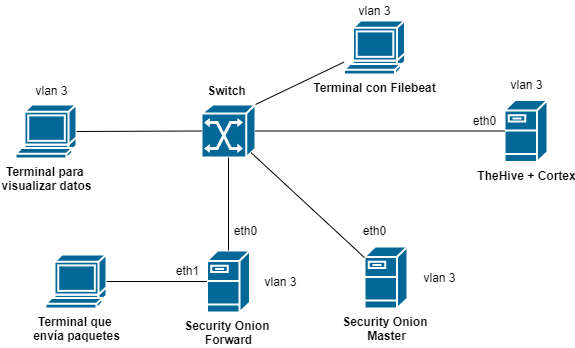
\includegraphics[width=1\textwidth]{./iteracion_1_imagenes/figura_33_c_topologia_de_prueba_3.png}
                \caption{Versión simplificada de la topología distribuida con todos sus componentes}
                \label{fig:topologia_distribuida_2}
            \end{figure}
            \FloatBarrier
            Luego de la incorporación de TheHive, se volvió a repetir el experimento detallado anteriormente, esta vez con el objetivo de que TheHive recibiera las alertas generadas en el nodo Master mediante ElastAlert. A diferencia del experimento anterior, en el que el nodo Master recibía logs filtrados desde Filebeat, en esta ocasión se lanzó al nodo Forward un ataque simulado por su interfaz de monitoreo.\par
            De esta manera, cuando el nodo Forward identificó el ataque, notificó al nodo Master del mismo. En el nodo Master, ElastAlert generó alertas que fueron enviadas al servidor de TheHive, quien las presentó a los analistas junto a información contextual que intentó correlacionar con información presente en su base de datos.\par
            %ACA CAMBIAR EL ARCHIVO Y NOMBRE DE LA FIGURA POR LA QUE ESTA CREANDO FEDE
            \begin{figure}[h]
            \centering
             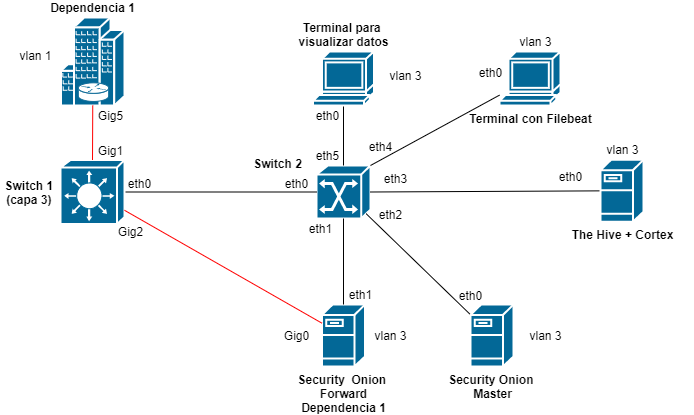
\includegraphics[width=1\textwidth]{./iteracion_1_imagenes/figura_33_d_topologia_de_prueba_4.png}
                \caption{Prueba de topología distribuida con trafico real}
              \label{fig:topologia_distribuida_4}
            \end{figure}
            \FloatBarrier
            Posteriormente, se procedió a reemplazar la terminal que, con el objetivo de simular ataques, enviaba paquetes al nodo Forward de Security Onion. El enlace que estaba conectado a esta terminal fue reemplazado por otro unido a un puerto de un switch Capa 3. Este dispositivo estaba, a su vez, conectado con una dependencia de la organización. Se repitió el experimento pero en lugar de tener un ataque simulado, el tráfico monitoreado por el nodo Forward procedía del tráfico real de la dependencia que era redirigido mediante el switch capa 3. La topología del experimiento mencionado se puede observar en la Figura (\ref{fig:topologia_distribuida_4}).\par
            Finalmente, se procedió a desplegar la configuración final de la topología de este proyecto. Esta consistió en agregar un segundo nodo Forward para monitorear el tráfico de una dependencia adicional, como se muestra en la Figura \ref{fig:topologia_despliegue_proyecto}.
            \par
            \begin{figure}[H]
                \centering
                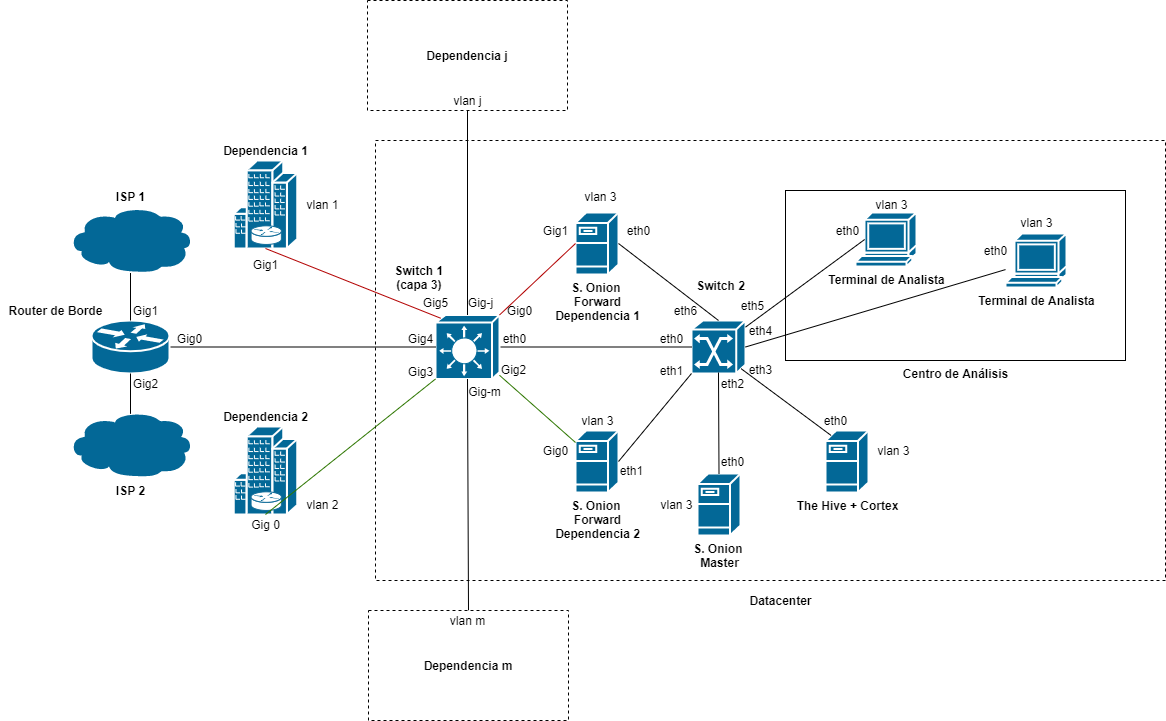
\includegraphics[width=1\textwidth]{./iteracion_1_imagenes/figura_33_arquitectura_despliegue_proyecto.png}
                \caption{Topología de Despliegue}
                \label{fig:topologia_despliegue_proyecto}
            \end{figure}
            \FloatBarrier
             La Figura \ref{fig:topologia_despliegue_proyecto} muestra la topología de prueba donde se instaló Security Onion. Se observan los proveedores de conexión a internet (ISP) y la conexión con el router de borde de la organización. Este último se conecta mediante un enlace gigabit en el puerto Gig0 al puerto Gig4 del switch 1 (capa 3). \par
             El switch 1 es un dispositivo de red de capa 3, que conecta las dependencias entre sí y con el datacenter. Las conexiones mencionadas se implementan físicamente sobre un enlace gigabit de fibra óptica, pero virtualmente sobre redes tipo VLAN. De esta manera, por ejemplo, la dependencia 1 está conectada físicamente por un enlace gigabit a través de su puerto Gig1 de su router de borde, con el puerto Gig5 del switch capa 3. Desde el punto de vista lógico, este enlace pertenece a la VLAN 1 de la organización. La situación descrita es análoga para el resto de las dependencias de la Universidad.\par
            Por otro lado, el switch 1 (en adelante SW 1), está conectado a los nodos Forward 1 y 2 de Security Onion. Como resultado, es posible reenviar el tráfico entre SW1 y las dependencias 1 y 2 hacia los puertos Gig0 y Gig2 de SW1 que conectan SW1 con los nodos Forward 1 y 2. \par
            SW1 está conectado con un switch 2 perteneciente al datacenter, al cual se conectan a su vez los terminales de los analistas, los nodos Master y Forward (1 y 2) de Security Onion y TheHive. Esta topología permite desplegar una arquitectura distribuida de Security Onion, que fue la elegida para este proyecto. 
        \end{subsection}

   \end{section}
    
    \begin{section}{Verificación de los requerimientos funcionales 1 y 3}
  
    \end{section}
   
   %\begin{section}{Configuración de acciones automáticas}
%        El mecanismo elegido para automatizar las acciones fue mediante webhooks, para ello fue necesario implementar un entorno de virtualización en el mismo servidor donde se encuentran alojados TheHive y Cortex. Para ello se optó por utilizar el módulo de python “venv”, lo que requirió la instalación de Python 3.6 como primer paso. En segundo lugar se modificó el archivo application.conf de TheHive que se mencionó en la sección anterior para permitir la comunicación con el puerto  del entorno de virtualización. En tercer lugar se verificó que en el nodo Master de Security Onion las reglas de ElastAlert tengan los campos necesarios configurados como observables ya que estos serán necesarios posteriormente dado que en TheHive están creados los observables que esperan esta información (source\_ip, destination\_ip, source\_port, destination\_port, alert, classification, category, etc). \par
%        Satisfechos los pasos anteriores, la instalación siguió los siguientes pasos:
%        \begin{itemize}
 %           \item Se creo una carpeta con el nombre webhooksenv
 %           \item Un entorno virtual fue creado y activado en la mencionada carpeta
 %           \item Se procedió a instalar las librerias necesarias: Flask, Gunicorn, Wheel, Request y Netaddr.
 %           \item Se desactivo el entorno virtual y se habilitó en el firewall el puerto 5000.
%            \item Se agregaron y modificaron valores al archivo de parámetros que utiliza webhooks.
%            \item Se inició y comprobó el estado del servicio.
%        \end{itemize}
%        Finalmente, se modificaron los archivos de configuración de TheHive y Cortex para actualizar la información necesaria referida a los webhooks.

   %\end{section}